\documentclass{article}
\usepackage[utf8]{inputenc}
\usepackage{macros}

\title{Literature}

\begin{document}
\maketitle

\section{Rademacher, 2005}
\cite{rademacher2005matrix} introduces fast approximate SVD via iterative sampling. They obtain bound
$$\norm{A - \tilde{A}_k}^2 \leq \frac{1}{1-\epsilon}\norm{A - A_k}^2 + \epsilon^t \norm{A}^2$$
with at least $3/4$ probability via iterative sampling, where $\tilde{A}_k$ is the sampled matrix. The first round of sampling samples row $i$ of $A$ with probability proportional to lengths squared. The second round of sampling samples row $i$ with probability proportional to the square of length of the residue of row $i$, after its projection onto the span of sampled rows. There are $t$ such rounds of sampling, with $k/\epsilon$ rows sampled each round. Thus, there are $tk/\epsilon$ rows in $\tilde{A}_k$. The algorithm \textbf{does not} compute the actual SVD of $A$, as opposed to the algorithm from \cite{drineas2007relativeerror}. Intuitively, if an important direction is not accounted for in round $i$, it will have a higher chance of being sampled in round $i+1$.

They also show existence of $4k^2/\epsilon$ rows that span matrix $\tilde{A}_k$ such that 
$$\norm{A - \tilde{A}_k}^2 \leq (1+\epsilon)\norm{A - A_k}^2 = (1+\epsilon)\opt.$$

Even though the claim itself is weaker than that in \cite{drineas2007relativeerror} (mere existence vs an algorithm finding it w.h.p.), the technique used is different from \cite{drineas2007relativeerror}, and can be of independent interest, In particular, this provides a certain guarantee of algorithm \ref{direct alg, M > 0}.

\section{Drineas, 2007}
\cite{drineas2007relativeerror} does matrix decomposition using rows of the matrix as principal vectors. They first \textbf{compute the SVD}, and then sample rows, s.t. row $i$ is sampled with probability proportional to the square of length of its projection onto the subspace spanned by principal vectors. They have two algorithms: one that samples $O(k\log k \log(1/\delta)/\epsilon^2)$ rows in expectation, and another that samples exactly $O(k^2\log(1/\delta)/\epsilon^2)$ rows 
They obtain multiplicative bound 
$$\norm{A - \tilde{A}_k}^2 \leq (1+\epsilon)\norm{A - A_k}^2 = (1+\epsilon)\opt$$ with probability at least $1-\delta$.

\section{Bernholt, 2004}
\cite{bernholt2004complexity} talks about minimum covariance determinant(MCD): they introduce an algorithm polynomial with running time $O(N^{\nu+1})$, where $\nu = d(d+3)/2$, and show that MCD is \textbf{NP}-hard if dimension $d$ varies.

\begin{definition}[MCD]
Let $\X\subset \R^d$ be a set of $N$ points. Given natural number $h$, the \textit{minimum covariance determinant problem} is to find an $h$-element subset $\X'\subset \X$ such that $\det{\X'}$ is minimal, where $\det{S}$ is the determinant of the matrix $SS^T$, where $S$ is both a set and a matrix, with columns from $S$. $(SS^T)_{d\times d}$ is the covariance matrix of $S$.
\end{definition}

\begin{definition}[Quadric]
A \textit{quadric} $Q$ in $\R^d$ is the set describable by a second-degree polynomial
\begin{equation}
    a_0 + \sum_{i=1}^d a_i z_i + 2\sum_{1\leq i< j\leq d} a_{i,j} z_i z_j + \sum_{i = 1}^d a_{i,i} z_i^2 = 0,
\end{equation}
where $a_i, a_{i,j}$ for $1\leq i\leq j\leq d$ are the coefficients defining the quadric, and $z = (z_1,...,z_d)\in \R^d$ is a point in $Q$.
Equivalently, it is the set $\set{z\in \R^d : z^T A z + z^T b + a_0 = 0}$, where $A_{i,j} = a_{i,j}$ is a symmetric matrix, and $b_i = a_i$ is a column vector. $Q$ is determined by $\nu+1$ parameters $a_0,...,a_d$,  $a_{i,j}$ for $1\leq i\leq j\leq d$, where $\nu = d(d+3)/2$. It is a generalization of an ellipsoid, and is a $(d-1)$-dimensional (smooth) manifold.
\end{definition}

An important fact they note in this paper is that selection by a quadric in $d$ dimensions is equivalent to selection by a hyperplane in $\nu$ dimensions. Indeed, consider the map $\mathbf{\widehat{}}: \R^d \to \R^\nu$ given by
$$\widehat{z} = (z_1,\dots,z_d, z_1z_1,\dots,z_iz_j,\dots,z_dz_d),\ 1\leq i\leq j\leq d.$$
Then the parameters $a_i,a_{i,j}$ define a hyperplane in $\R^\nu$ with the property that 
$$ \text{$z$ selected by quadric $Q \iff \widehat{z} $ is selected by the hyperplane$ \iff \inp{\widehat{z}}{\widehat{a}} + a_0\leq 0$}, $$
where $\widehat{a} = (a_1,\dots,a_d, a_{1,1},\dots,a_{i,j},\dots,a_{d,d})$

Since by \cite{rousseeuw1999fast} we know that a set that solves MCD is selectable by an ellipsoid, it is enough to find an ellipsoid that selects the optimal set. They show that any set selectable by an ellipsoid is (almost) selectable by a quadric with the coefficients $a_i, a_{i,j} \subset \X$, and there are $O(N^{\nu+1})$ of those. The precise statement is

\begin{theorem}
Given a solid ellipsoid $E$, let $\X' = E\cap \X$, so $\X'$ is selected by $E$. Then there exists set $S\subset \X$ of $\nu := d(d+3)/2$ elements such that for the quadric defined by $A, b, a_0$ we have
\begin{align*}
x^TAx + x^Tb + a_0 \leq 0 &\text{ for all $x\in \X'$}\\
x^TAx + x^Tb + a_0 \geq 0 &\text{ for all $x\in \X\setminus\X'$}.
\end{align*}
The proof comes from the fact that separation by a quadric in $\R^d$ is equivalent to separation by a hyperplane in $\R^\nu$ by mapping all $x\in \R^d$ to $\hat{x} = (x_1,...,x_d,x_{1,1},..., x_{i,j},...,x_{d,d})\in \R^\nu, 1\leq i\leq j \leq d$.

So it is enough to check all subsets of $\X$ of size $\nu$ to uncover the quadric selecting the optimal set (gotta be careful about the boundary terms $x$ s.t. $x^TAx + x^Tb + a_0 = 0$ but it works out).

\end{theorem}

\section{Rousseeuw, 1999}
\cite{rousseeuw1999fast} shows that any subset that minimizes the covariance determinant is selectable by an ellipsoid (corollary 1). 

They also introduce a C-step, which, given a set, will find a new set with smaller or equal covariance determinant. It is done by selecting the $h$ elemens with the smallest Mahalanobis distance.

Additionally, they present a fast algorithm for approximating MCD, which is iterative and finds a local optimum. They run a lot of randomly initialized parallel computations as an attempt to find the global optimum.

Their algorithm is to initialize a lot of subsets $\X'$ of the original set $\X$, and apply C-steps to each one until convergence. To initialize, for each subset $\X'$ they select $k$ values u.i.r., compute the covariance matrix, and add $n-k$ values from $\X$ that have the lowest Mahalanobis distance.

\section{chawla, 2013}
\cite{chawla2013k} introduce k-means--, which works with outliers. They claim that for $k=1, \ell>1$, k-means-- is a special case of MCD. This is true because the set $\X' = \X \setminus \text{\{outliers\}}$ is selectable by an ellipsoid (a sphere, in fact). 

\section{Hubert and Rousseeuw, 2005}
\cite{hubert2005robpca} consider a problem quite similar to ours: given a set $\X \subset \R^d$ and integers $k$ and $0.5 |\X| \leq h$, find a subset of $\X$ of size $h$ that has the best PCA approximation. Unfortunately, they never actually state the problem precisely, so it is unclear how they measure the goodness of PCA approximation of a set. Their algorithm is quite convoluted, but is quite different from all algorithms we have thought of for our problem. A big difference between their problem and ours is that their require $0.5 |\X| \leq h$, and think of all elements that are discarded as outliers. We, on the other hand, might choose $h$ to be small, and think of the chosen points as a community, without labeling all other points as outliers.

In their algorithm they use a measure of ''outlyingness`` for each point to select those are are not outliers. It is given by 
$$\text{outl}_A(x_i) = \max_{v\in B} \frac{|x_i^T v - \text{med}(x_j^T v)|}{\text{mad}(x_j^T v)},$$
where $B$ contains all non-zero vectors, $\text{med}(x_j^T v)$ is the median of $\set{x_j^T v : x_j \in \X}$, and $\text{mad}(x_j^T v) = \text{med}|x_j^T v - \text{med}(x_{\ell}^T v)|.$

\section{Candes, 2011, Robust PCA}
\cite{candes2011robust} describes an algorithm to find low-rank $L_0$ and sparse $N_0$ given $M_{n_1 \times n_2} = L_0 + N_0$. They assume the incoherence condition with parameter $\mu$, which is that for $L_0 = U\Sigma V^* = \sum_{i=1}^r \sigma_i u_i v_i^*,$ the following hold:
\begin{equation}\label{eqn: incoherence conditions}
    \max_i \norm{U^* e_i}^2 \leq \frac{\mu r}{n_1},\hspace{0.5cm} \max_i \norm{V^* e_i}^2 \leq \frac{\mu r}{n_2},\hspace{0.5cm} \norm{U V^*}_\infty \leq \sqrt{\frac{\mu r}{n_1 n_2}},
\end{equation}
where $\norm{.}_\infty$ is the $\ell_\infty$ norm, i.e. the largest absolute value, and $\norm{.}$ is the Frobenius norm. The incoherence condition \ref{eqn: incoherence conditions} ensures that singular vectors are not sparse, i.e. their entries are more or less uniform in absolute value.

They solve the optimization problem
\begin{align*}
    \text{minimize }& \norm{L}_* + \lambda \norm{S}_1\\
    \text{subject to }& L+S = M,
\end{align*}
which under specific conditions provides an \textit{exact} solution.

This is the main theorem:
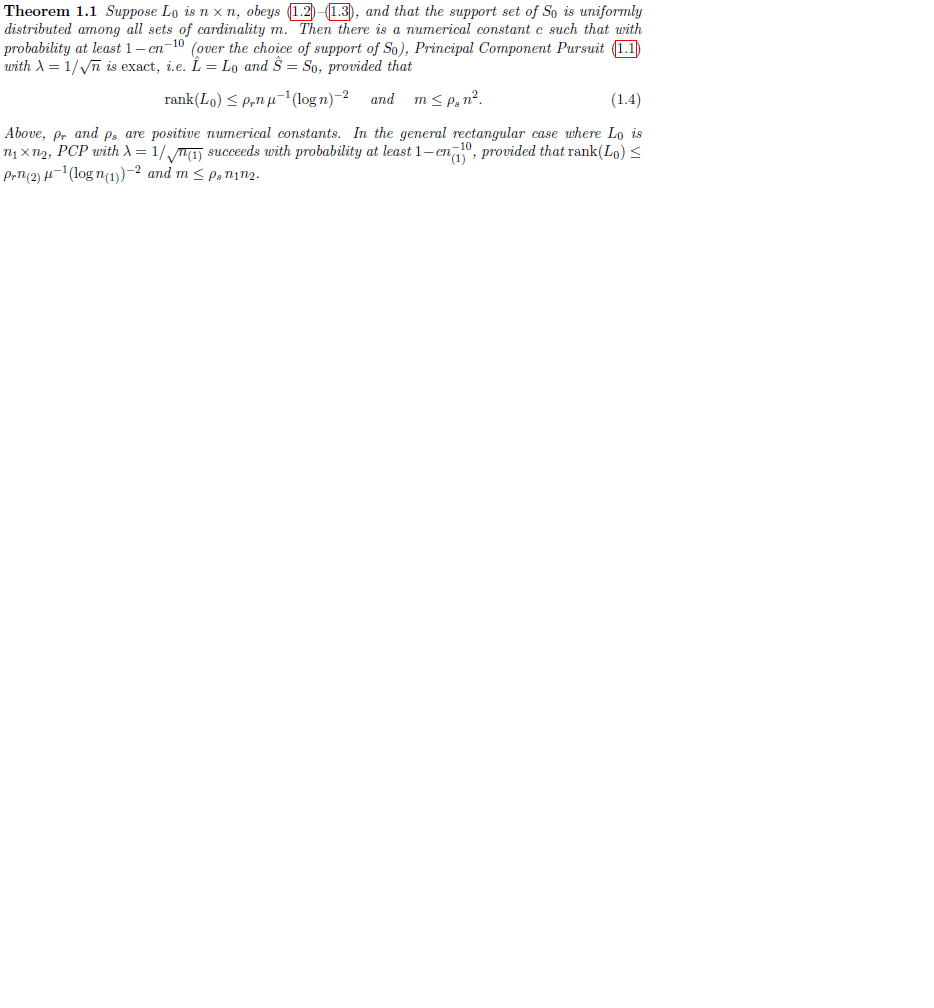
\includegraphics[]{images/theorem1_1.png}


\printbibliography

\end{document}